\underrubrik{Vi vill att du p{\aa}verkar vad som h{\"a}nder p{\aa} scen!}
\begingroup
\fontsize{11}{13}\selectfont
\parskip=0.5\baselineskip
G{\"o}r inrop!
I F-spexet {\"a}r det publiken som best{\"a}mmer genom att ropa hur skådespelarna ska agera. Har du en kul id{\'e} s{\aa} tveka inte att ropa till skådespelarna!

\underrubrik{Inropsbingo}
Om du vill ha lite mer utmaning kan du spela inropsbingo med en kompis. 
Innan f{\"o}rest{\"a}llningen b{\"o}rjar byter ni program med varandra och fyller i varandras spelplan, ett rop per ruta. Kom ih{\aa}g att s{\"a}ga ett pris ocks{\aa}, till exempel vem som skall k{\"o}pa l{\"a}sk i aktpausen.

N{\"a}r f{\"o}rest{\"a}llningen v{\"a}l har b{\"o}rjat kan ni eller andra i lokalen ropa och det {\"a}r till{\aa}tet att ropa saker fr{\aa}n sin egen bricka.  Om n{\aa}gon (t ex du) ropar det som st{\aa}r p{\aa} din bricka, och skådespelarna reagerar, s{\aa} kan den rutan p{\aa} brickan kryssas av. F{\"o}rst till 5 i rad ropar naturligtvis \citat{bingo}!

%\begin{multicols}{2}
%\begin{itemize}[labelwidth=7pt,leftmargin=!]\raggedright
%\item H{\"o}gre!
%\item H{\aa}rdare!
%\item Starkare!
%\item Mer psykedeliskt!
%\item Byt dialekt!
%\item Blygare!
%\item Som Kungen!
%\item Som en person som gjort bort sig!
%\item Varmare!
%\item Manligare/kvinnligare!
%\item Prata bakl{\"a}nges!
%\item Byt roller!
%\item Som en chalmersprofessor!
%\item Mer ordvitsar!
%\item Galnare!
%\item D{\"o}dare!
%\item P{\aa} norska!
%\item I falsett!
%\end{itemize}
%\end{multicols}
%
%

%\rubrik{Hur du f{\aa}r mer kupletter!}
%\lettrine[lines=3]{N}{{\"a}r} du minst anar det kommer folk p{\aa} scen bryta ut i s{\aa}ng till orkesterns ljuva ljud. 
%Om du tycker om kupletten kan du klappa ivrigt f{\"o}r att uppmuntra spexarna att framf{\"o}ra ytterligare en kuplett. 
%Om du tycker att kupletten var lite s{\aa} d{\"a}r, uppmuntra dem {\"a}nnu mer, s{\aa} kommer de framf{\"o}ra en ny version som ni tycker b{\"a}ttre om.
\begingroup\fontsize{10}{12}\selectfont


\begin{center}
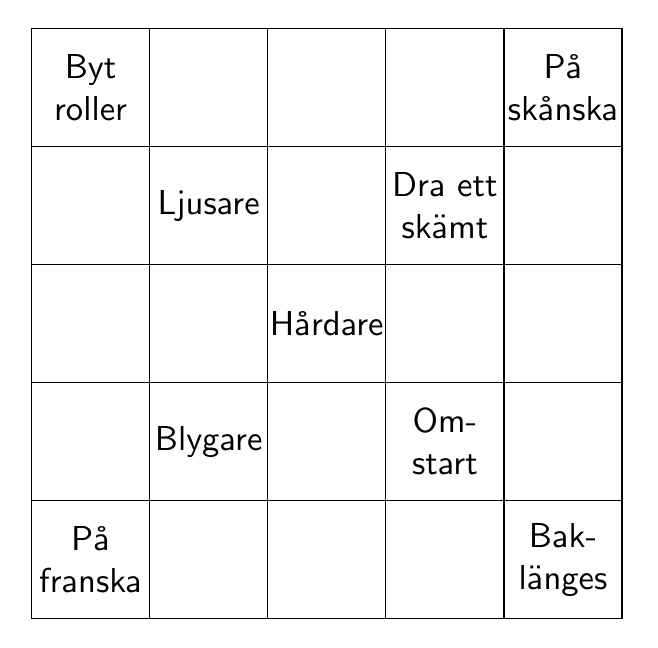
\begin{tikzpicture}[>=latex]
\tikzstyle{every node}=[font=\sf,align=center,scale=1.25]
\draw[step=1.5cm,color=black] (0,0) grid (7.5,7.5);
\node at (6.75,0.75) {Bak-\\l{\"a}nges};
\node at (5.25,2.25) {Om-\\start};
\node at (2.25,5.25) {Ljusare};
\node at (0.75,6.75) {Byt\\ roller};
\node at (6.75,6.75) {P{\aa} \\ sk{\aa}nska};
\node at (5.25,5.25) {Dra ett \\ sk{\"a}mt};
\node at (3.75,3.75) {H{\aa}rdare};
\node at (2.25,2.25) {Blygare};
\node at (0.75,0.75) {P{\aa}\\ franska};
\end{tikzpicture}
\end{center}

\endgroup
\endgroup

